\documentclass[12pt]{article}
\usepackage{graphicx}
\usepackage{amsmath}
\usepackage{mathtools}
\usepackage{gensymb}
\usepackage[utf8]{inputenc}
\usepackage{float}
\providecommand{\brak}[1]{\ensuremath{\left(#1\right)}}
%\providecommand{\norm}[1]{\left\lVert#1\right\rVert}
\newcommand{\solution}{\noindent \textbf{Solution: }}
\usepackage{atbegshi}% http://ctan.org/pkg/atbegshi
\AtBeginDocument{\AtBeginShipoutNext{\AtBeginShipoutDiscard}}
\let\vec\mathbf
\begin{document}
\begin{center}
\title{\textbf{STRAIGHT LINES}}
\maketitle
\end{center}
\begin{enumerate}
\item\textbf{Problem statement :} Find the slope of a line, which makes an angle of $30^\circ$ with positive direction of y-axis measured anticlockwise

\solution
\\
The slope m of a line making an angle $\theta$ with the positive direction of x axis in anticlockwise direction is given by,
\begin{align}
    m=\tan\theta
\end{align}
The angle made by the line with the positive direction of x-axis in anticlockwise direction is,
\begin{align}
    \theta=90\degree + 30\degree=120\degree
\end{align}
Substitute the value of $\theta$ in equation (1)
\begin{align}
        m=\tan120\degree = -\sqrt{3}
\end{align}
\begin{figure}[!h]
 \begin{center}
  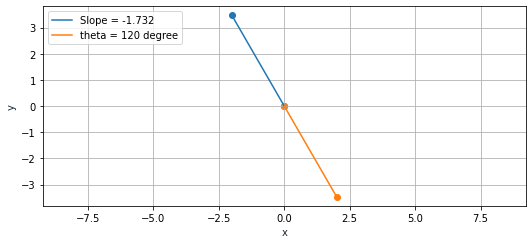
\includegraphics[width=\columnwidth]{figs/fig.png}
 \end{center}
\caption{}
\label{fig:Fig1}
\end{figure}
\end{enumerate}
\end{document}
